\clearpage

\section{Transparent with 1+1 Protection}\label{ILP_Transp_Protection}

\subsection{Model description}

Once more, to apply the ILP model we have to take into account the physical and logical topologies allowed by this mode of transport and the type of survivability. Through the following figures it is possible to see these topologies.\\

\begin{figure}[h!]
\centering
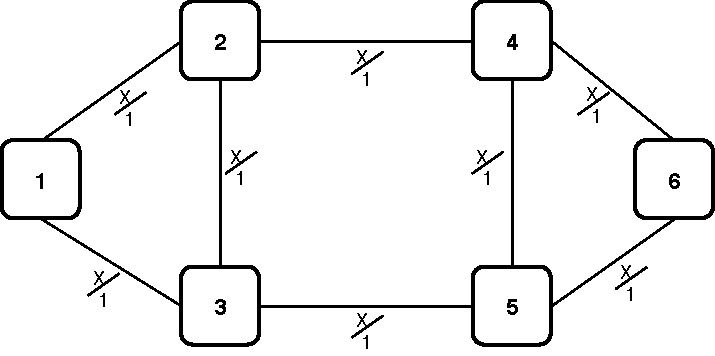
\includegraphics[width=12cm]{sdf/ilp/transparent_protection/figures/allowed_physical_topology}
\caption{Transparent with 1+1 protection: Allowed physical topology. The allowed physical topology is defined by the duct and sites in the field. It is assumed that each duct supports up to 1 bidirectional transmission system and each site supports up to 1 node.}
\label{allowed2_physical_protectionlow}
\end{figure}

\vspace{15pt}
\begin{figure}[h!]
\centering
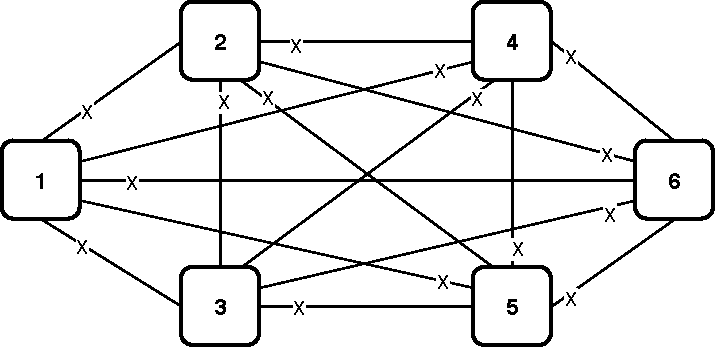
\includegraphics[width=11cm]{sdf/ilp/transparent_protection/figures/allowed_optical_topology}
\caption{Transparent with 1+1 protection: Allowed optical topology. The allowed optical topology is defined by the transport mode (transparent transport mode in this case). It is assumed that each connections between demands supports up to 100 lightpaths.}
\label{allowed2_optical_protectionlow}
\end{figure}

Now taking this into consideration and based on the specific constraints of the transparent mode with 1+1 protection it is possible to define the ILP model.\\
\newpage
The objective function, to be minimized, is the expression \ref{ILPOpaque_CAPEX}, i.e.,
\begin{equation*}
  minimize \qquad \Big\{ \quad C_C \quad \Big\}
\end{equation*}

$subject$ $to$
\begin{equation}
\sum_{c\in C} B\left(c\right) D_{odc} \leq \tau \lambda_{od} \qquad \qquad \qquad \qquad \qquad \qquad \qquad \qquad \qquad \qquad
\forall(o,d) : o < d
\label{ILPTransp0}
\end{equation}
\noindent
This restriction is considered grooming constraint and for this model the grooming can be done before routing since the traffic is aggregated just for demands between the same nodes, thus not depending on the routes. The variable  $\tau$ is always 100 Gbits/s.

\begin{equation}
\sum_{j\textbackslash \{o\}} f_{ij}^{od} = \lambda_{od} \qquad \qquad \qquad \qquad \qquad \qquad \qquad \qquad \qquad
\forall(o,d) : o < d, \forall i: i = o
\label{ILPTransp1}
\end{equation}
\noindent
This constraint is equal to the constraint \ref{ILPOpaque1_CAPEX} assuming that Z variable has the value of number of optical channels between this demand for all bidirectional links.

\begin{equation}
\sum_{j\textbackslash \{o\}} f_{ij}^{od} = \sum_{j\textbackslash \{d\}} f_{ji}^{od} \qquad \qquad \qquad \qquad \qquad \qquad \qquad \qquad
\forall(o,d) : o < d, \forall i: i \neq o,d
\label{ILPTransp2}
\end{equation}
\noindent
This constraint is equal to the constraint \ref{ILPOpaque2_CAPEX}.

\begin{equation}
\sum_{j\textbackslash \{d\}} f_{ji}^{od} = \lambda_{od}  \qquad \qquad \qquad \qquad \qquad \qquad \qquad \qquad \qquad
\forall(o,d) : o < d, \forall i: i = d
\label{ILPTransp3}
\end{equation}
\noindent
This constraint is equal to the constraint \ref{ILPOpaque3_CAPEX} assuming that Z variable has the value of number of optical channels between this demand for all bidirectional links.

\begin{equation}
\sum_{j\textbackslash \{o\}} fp_{ij}^{od} = \lambda_{od} \qquad \qquad \qquad \qquad \qquad \qquad \qquad \qquad \qquad
\forall(o,d) : o < d, \forall i: i = o
\label{ILPTransp1p}
\end{equation}
\noindent
This is the protection flow conservation constraints and ensure that, for each $(o,d)$ pair, we route the number of optical channels of flow from node $o$ to node $d$, the source node sends the number of optical channels units of flow.
\newpage
\begin{equation}
\sum_{j\textbackslash \{o\}} fp_{ij}^{od} = \sum_{j\textbackslash \{d\}} fp_{ji}^{od} \qquad \qquad \qquad \qquad \qquad \qquad \qquad
\forall(o,d) : o < d, \forall i: i \neq o,d
\label{ILPTransp2p}
\end{equation}
\noindent
This constraint ensure that the remaining nodes, being neither origin or destination, the receive flow have to be send.

\begin{equation}
\sum_{j\textbackslash \{d\}} fp_{ji}^{od} = \lambda_{od} \qquad \qquad \qquad \qquad \qquad \qquad \qquad \qquad \qquad
\forall(o,d) : o < d, \forall i: i = d
\label{ILPTransp3p}
\end{equation}
\noindent
This is the protection flow conservation constraints and ensure that, for each $(o,d)$ pair, we route the number of optical channels units of flow from node $o$ to node $d$, the destination node has to receive those the number of optical channels units of flow.

\begin{equation}
\sum_{o=1} \sum_{d=o+1} \left(f_{ij}^{od}  + fp_{ij}^{od}\right) \leq \lambda_{od}  \qquad \qquad \qquad \qquad \qquad \qquad \qquad \qquad \qquad
\forall (o,d), (i,j)
\label{ILPTransp4p}
\end{equation}
\noindent
This constraint assures us that the variable $f_{ij}^{od}$ (working flow) and $fp_{ij}^{od}$ (protection flow) are different.

\begin{equation}
\sum_{o=1} \sum_{d=o+1} \left(f_{ij}^{od} + f_{ji}^{od} + fp_{ij}^{od} + fp_{ji}^{od}\right) \leq K_{ij} G_{ij} L_{ij} \qquad \qquad \qquad \qquad
\forall(i,j) : i < j
\label{ILPTransp4}
\end{equation}
\noindent
This restriction answers capacity constraint problem. Then, total flows must be less or equal to the capacity of network links. For any situation the maximum number of optical channels supported by each transmission system is 100, i.e., $K_{ij}$ = 100.

\begin{equation}
f_{ij}^{od} , f_{ji}^{od} , fp_{ij}^{od} , fp_{ji}^{od} , \lambda_{od} \in \mathbb{N}   \qquad \qquad \qquad \qquad \qquad
\forall(i,j) : i < j, \forall(o,d) : o < d
\label{ILPTransp5}
\end{equation}
\noindent
This constraint define the total number of flows and the number of optical channels must be a counting number.

\begin{equation}
L_{i,j} \in \{0,1\} \qquad \qquad \qquad \qquad \qquad \qquad \qquad \qquad \qquad \qquad \qquad \qquad \qquad \qquad
\forall(i,j)
\label{ILPTranspL1}
\end{equation}
\noindent
Last constraint refers to the use of the link where this variable can be zero if it is not being used or one if is being used.

\subsection{Result description}

\textbf{Low Traffic Scenario:}\\

In this scenario we have to take into account the traffic calculated in \ref{low_scenario}. In a first phase, we will show the resulting physical and optical topology. These topologies are based on the allowed topologies referred to in the model description and also taking into account the logical topology for all ODUs mentioned in the section \ref{low_scenario}.\\

\begin{figure}[h!]
\centering
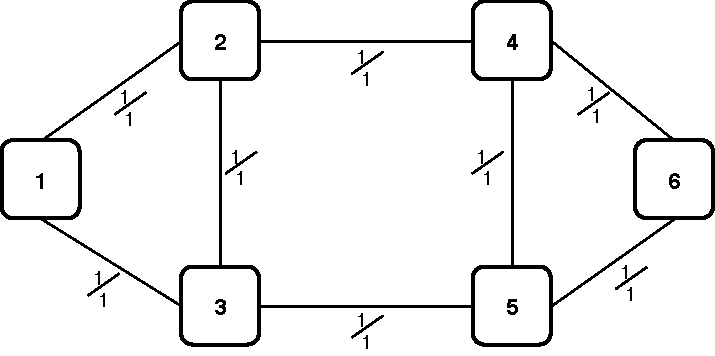
\includegraphics[width=12cm]{sdf/ilp/transparent_protection/figures/physical_topology}
\caption{Transparent with 1+1 protection in low scenario: Physical topology after dimensioning.}
\label{physical2_protectionlow}
\end{figure}

\vspace{15pt}
\begin{figure}[h!]
\centering
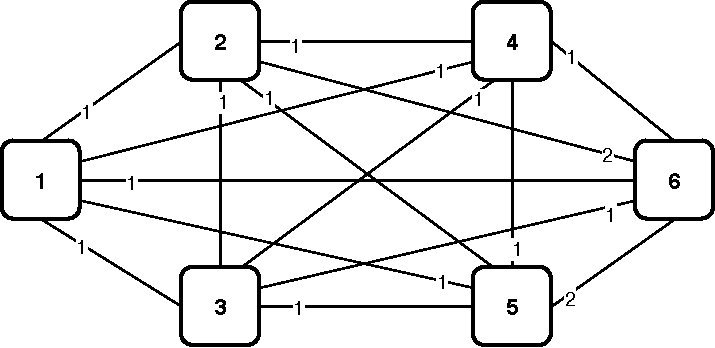
\includegraphics[width=12cm]{sdf/ilp/transparent_protection/figures/optical_topology_low}
\caption{Transparent with 1+1 protection in low scenario: Optical topology after dimensioning.}
\label{optical2_protectionlow}
\end{figure}
\newpage
In table \ref{link_transp_protec_ref_low} we can see the number of optical channels calculated using \ref{Capex_Link} and \ref{ILPOpaque_CAPEX} and the number of amplifiers for each link calculated using \ref{Capex_amplifiers}.\\

\begin{table}[h!]
\centering
\begin{tabular}{|| c | c | c ||}
 \hline
 \multicolumn{3}{|| c ||}{Information regarding links} \\
 \hline
 \hline
 Bidirectional Link & Optical Channels & Amplifiers\\
 \hline
 Node 1 <-> Node 2 & 6 & 4 \\
 Node 1 <-> Node 3 & 6 & 6 \\
 Node 2 <-> Node 3 & 10 & 0 \\
 Node 2 <-> Node 4 & 10 & 6 \\
 Node 3 <-> Node 5 & 10 & 8 \\
 Node 4 <-> Node 5 & 10 & 1 \\
 Node 4 <-> Node 6 & 8 & 7 \\
 Node 5 <-> Node 6 & 8 & 3 \\
 \hline
\end{tabular}
\caption{Table with information regarding links for transparent mode with 1+1 protection in low scenario.}
\label{link_transp_protec_ref_low}
\end{table}

In table \ref{node_transp_protec_ref_low} we can see the resulting nodal degree at the physical layer, the number of line ports and the number of add ports for the optical part calculated using \ref{OXC_poxc_transparent} the number of LR transponders calculated using \ref{EXC_pexc2_transparent} and the number of tributary ports calculated using \ref{EXC_pexc1_transparent} for each node.\\

\begin{table}[h!]
\centering
\begin{tabular}{|| c | c | c | c | c | c ||}
 \hline
 \multicolumn{6}{|| c ||}{Information regarding nodes} \\
 \hline
 \hline
 \multicolumn{2}{|| c |}{ } & \multicolumn{2}{ c |}{Electrical part} & \multicolumn{2}{ c ||}{Optical part} \\
 \hline
 Node & Resulting Nodal Degree & Tributary Ports & LR Transponders & Add Ports & Line Ports\\
 \hline
 1 & 2 & 29 & 5 & 5 & 12 \\
 2 & 3 & 23 & 6 & 6 & 26 \\
 3 & 3 & 18 & 5 & 5 & 26 \\
 4 & 3 & 20 & 5 & 5 & 28 \\
 5 & 3 & 24 & 6 & 6 & 28 \\
 6 & 2 & 22 & 7 & 7 & 16 \\
\hline
\end{tabular}
\caption{Table with information regarding nodes for transparent mode with 1+1 protection in low scenario.}
\label{node_transp_protec_ref_low}
\end{table}
\newpage
Through the information obtained previously on the nodes we can now create tables with detailed information about each node.
\begin{table}[h!]
\centering
\begin{tabular}{|| c | c | c ||}
 \hline
 \multicolumn{3}{|| c ||}{Detailed description of Node 1} \\
 \hline
 \hline
 Electrical part & Number of tributary ports & Bit rate \\ \hline
\multirow{3}{*}{29 tributary ports} & 13 & ODU0 \\
 & 13 & ODU1 \\
 & 3 & ODU2 \\
 \hline
  & Node<--Optical Channels-->Node & Bit rate \\
 \hline
 \multirow{5}{*}{5 LR Transponders} & 1  <---- 1 ---->  2 & \multirow{5}{*}{100 Gbits/s} \\
  & 1  <---- 1 ---->  3 & \\
  & 1  <---- 1 ---->  4 & \\
  & 1  <---- 1 ---->  5 & \\
  & 1  <---- 1 ---->  6 & \\
 \hline
 \hline
 Optical part & Node<--Optical Channels-->Node & Bit rate \\
 \hline
 \multirow{5}{*}{5 add ports} & 1  <---- 1 ---->  2 & \multirow{11}{*}{100 Gbits/s} \\
  & 1  <---- 1 ---->  3 & \\
  & 1  <---- 1 ---->  4 & \\
  & 1  <---- 1 ---->  5 & \\
  & 1  <---- 1 ---->  6 & \\ \cline{1-2}
 \multirow{6}{*}{12 line ports} & 1  <---- 1 ---->  2 & \\
  & 1  <---- 1 ---->  3 & \\
  & 1  <---- 1 ---->  4 & \\
  & 1  <---- 1 ---->  5 & \\
  & 1  <---- 1 ---->  6 & \\
  & 2  <---- 1 ---->  3 & \\
\hline
\end{tabular}
\caption{Transparent with 1+1 protection in low scenario: Detailed description of node 1. The number of demands is distributed to the various destination nodes, this distribution can be observed in section \ref{low_scenario}. Regarding the number of line ports when this node is equal to the source, it means that add ports are used, otherwise it means that through ports are used.}
\end{table}

\newpage
\begin{table}[h!]
\centering
\begin{tabular}{|| c | c | c ||}
 \hline
 \multicolumn{3}{|| c ||}{Detailed description of Node 2} \\
 \hline
 \hline
 Electrical part & Number of tributary ports & Bit rate \\ \hline
\multirow{5}{*}{23 tributary ports} & 11 & ODU0 \\
 & 7 & ODU1 \\
 & 2 & ODU2 \\
 & 2 & ODU3 \\
 & 1 & ODU4 \\
 \hline
  & Node<--Optical Channels-->Node & Bit rate \\
 \hline
 \multirow{5}{*}{6 LR Transponders} & 2  <---- 1 ---->  1 & \multirow{5}{*}{100 Gbits/s}\\
  & 2  <---- 1 ---->  3 & \\
  & 2  <---- 1 ---->  4 & \\
  & 2  <---- 1 ---->  5 & \\
  & 2  <---- 2 ---->  6 & \\
 \hline
 \hline
 Optical part & Node<--Optical Channels-->Node & Bit rate \\
 \hline
 \multirow{5}{*}{6 add ports} & 2  <---- 1 ---->  1 & \multirow{17}{*}{100 Gbits/s} \\
  & 2  <---- 1 ---->  3 & \\
  & 2  <---- 1 ---->  4 & \\
  & 2  <---- 1 ---->  5 & \\
  & 2  <---- 2 ---->  6 & \\ \cline{1-2}
 \multirow{12}{*}{26 line ports} & 2  <---- 1 ---->  1 & \\
  & 2  <---- 1 ---->  3 & \\
  & 2  <---- 1 ---->  4 & \\
  & 2  <---- 1 ---->  5 & \\
  & 2  <---- 2 ---->  6 & \\
  & 1  <---- 1 ---->  3 & \\
  & 1  <---- 1 ---->  4 & \\
  & 1  <---- 1 ---->  5 & \\
  & 1  <---- 1 ---->  6 & \\
  & 3  <---- 1 ---->  4 & \\
  & 3  <---- 1 ---->  5 & \\
  & 3  <---- 1 ---->  6 & \\
\hline
\end{tabular}
\caption{Transparent with 1+1 protection in low scenario: Detailed description of node 2. The number of demands is distributed to the various destination nodes, this distribution can be observed in section \ref{low_scenario}. Regarding the number of line ports when this node is equal to the source, it means that add ports are used, otherwise it means that through ports are used. In both cases the number of ports is double the number of optical channels.}
\end{table}

\newpage
\begin{table}[h!]
\centering
\begin{tabular}{|| c | c | c ||}
 \hline
 \multicolumn{3}{|| c ||}{Detailed description of Node 3} \\
 \hline
 \hline
 Electrical part & Number of tributary ports & Bit rate \\ \hline
\multirow{4}{*}{18 tributary ports} & 7 & ODU0 \\
 & 6 & ODU1\\
 & 3 & ODU2\\
 & 2 & ODU3\\
 \hline
  & Node<--Optical Channels-->Node & Bit rate \\
 \hline
 \multirow{5}{*}{5 LR Transponders} & 3  <---- 1 ---->  1 & \multirow{5}{*}{100 Gbits/s} \\
  & 3  <---- 1 ---->  2 & \\
  & 3  <---- 1 ---->  4 & \\
  & 3  <---- 1 ---->  5 & \\
  & 3  <---- 1 ---->  6 & \\
 \hline
 \hline
 Optical part & Node<--Optical Channels-->Node & Bit rate \\
 \hline
 \multirow{5}{*}{5 add ports} & 3  <---- 1 ---->  1 & \multirow{17}{*}{100 Gbits/s} \\
  & 3  <---- 1 ---->  2 & \\
  & 3  <---- 1 ---->  4 & \\
  & 3  <---- 1 ---->  5 & \\
  & 3  <---- 1 ---->  6 & \\ \cline{1-2}
 \multirow{12}{*}{26 line ports} & 3  <---- 1 ---->  1 & \\
  & 3  <---- 1 ---->  2 & \\
  & 3  <---- 1 ---->  4 & \\
  & 3  <---- 1 ---->  5 & \\
  & 3  <---- 1 ---->  6 & \\
  & 1  <---- 1 ---->  2 & \\
  & 1  <---- 1 ---->  4 & \\
  & 1  <---- 1 ---->  5 & \\
  & 1  <---- 1 ---->  6 & \\
  & 2  <---- 1 ---->  4 & \\
  & 2  <---- 1 ---->  5 & \\
  & 2  <---- 2 ---->  6 & \\
\hline
\end{tabular}
\caption{Transparent with 1+1 protection in low scenario: Detailed description of node 3. The number of demands is distributed to the various destination nodes, this distribution can be observed in section \ref{low_scenario}. Regarding the number of line ports when this node is equal to the source, it means that add ports are used, otherwise it means that through ports are used. In both cases the number of ports is double the number of optical channels.}
\end{table}

\newpage
\begin{table}[h!]
\centering
\begin{tabular}{|| c | c | c ||}
 \hline
 \multicolumn{3}{|| c ||}{Detailed description of Node 4} \\
 \hline
 \hline
 Electrical part & Number of tributary ports & Bit rate \\ \hline
\multirow{3}{*}{20 tributary ports} & 7 & ODU0 \\
 & 10 & ODU1 \\
 & 3 & ODU2 \\
 \hline
  & Node<--Optical Channels-->Node & Bit rate \\
 \hline
 \multirow{5}{*}{5 LR Transponders} & 4  <---- 1 ---->  1 & \multirow{5}{*}{100 Gbits/s} \\
  & 4  <---- 1 ---->  2 & \\
  & 4  <---- 1 ---->  3 & \\
  & 4  <---- 1 ---->  5 & \\
  & 4  <---- 1 ---->  6 & \\
 \hline
 \hline
 Optical part & Node<--Optical Channels-->Node & Bit rate \\
 \hline
 \multirow{5}{*}{5 add ports} & 4  <---- 1 ---->  1 & \multirow{17}{*}{100 Gbits/s} \\
  & 4  <---- 1 ---->  2 & \\
  & 4  <---- 1 ---->  3 & \\
  & 4  <---- 1 ---->  5 & \\
  & 4  <---- 1 ---->  6 & \\ \cline{1-2}
 \multirow{12}{*}{28 line ports} & 4  <---- 1 ---->  1 & \\
  & 4  <---- 1 ---->  2 & \\
  & 4  <---- 1 ---->  3 & \\
  & 4  <---- 1 ---->  5 & \\
  & 4  <---- 1 ---->  6 & \\
  & 1  <---- 1 ---->  5 & \\
  & 1  <---- 1 ---->  6 & \\
  & 2  <---- 1 ---->  5 & \\
  & 2  <---- 2 ---->  6 & \\
  & 3  <---- 1 ---->  5 & \\
  & 3  <---- 1 ---->  6 & \\
  & 5  <---- 2 ---->  6 & \\
\hline
\end{tabular}
\caption{Transparent with 1+1 protection in low scenario: Detailed description of node 4. The number of demands is distributed to the various destination nodes, this distribution can be observed in section \ref{low_scenario}. Regarding the number of line ports when this node is equal to the source, it means that add ports are used, otherwise it means that through ports are used. In both cases the number of ports is double the number of optical channels.}
\end{table}

\newpage
\begin{table}[h!]
\centering
\begin{tabular}{|| c | c | c ||}
 \hline
 \multicolumn{3}{|| c ||}{Detailed description of Node 5} \\
 \hline
 \hline
 Electrical part & Number of tributary ports & Bit rate \\ \hline
\multirow{5}{*}{24 tributary ports} & 14 & ODU0 \\
 & 4 & ODU1 \\
 & 4 & ODU2 \\
 & 1 & ODU3 \\
 & 1 & ODU4 \\
 \hline
  & Node<--Optical Channels-->Node & Bit rate \\
 \hline
 \multirow{5}{*}{6 LR Transponders} & 5  <---- 1 ---->  1 & \multirow{5}{*}{100 Gbits/s} \\
  & 5  <---- 1 ---->  2 & \\
  & 5  <---- 1 ---->  3 & \\
  & 5  <---- 1 ---->  4 & \\
  & 5  <---- 2 ---->  6 & \\
 \hline
 \hline
 Optical part & Node<--Optical Channels-->Node & Bit rate \\
 \hline
 \multirow{5}{*}{6 add ports} & 5  <---- 1 ---->  1 & \multirow{17}{*}{100 Gbits/s} \\
  & 5  <---- 1 ---->  2 & \\
  & 5  <---- 1 ---->  3 & \\
  & 5  <---- 1 ---->  4 & \\
  & 5  <---- 2 ---->  6 & \\ \cline{1-2}
 \multirow{12}{*}{28 line ports} & 5  <---- 1 ---->  1 & \\
  & 5  <---- 1 ---->  2 & \\
  & 5  <---- 1 ---->  3 & \\
  & 5  <---- 1 ---->  4 & \\
  & 5  <---- 2 ---->  6 & \\
  & 1  <---- 1 ---->  4 & \\
  & 1  <---- 1 ---->  6 & \\
  & 2  <---- 1 ---->  4 & \\
  & 2  <---- 2 ---->  6 & \\
  & 3  <---- 1 ---->  4 & \\
  & 3  <---- 1 ---->  6 & \\
  & 4  <---- 1 ---->  6 & \\
\hline
\end{tabular}
\caption{Transparent with 1+1 protection in low scenario: Detailed description of node 5. The number of demands is distributed to the various destination nodes, this distribution can be observed in section \ref{low_scenario}. Regarding the number of line ports when this node is equal to the source, it means that add ports are used, otherwise it means that through ports are used. In both cases the number of ports is double the number of optical channels.}
\end{table}

\newpage
\begin{table}[h!]
\centering
\begin{tabular}{|| c | c | c ||}
 \hline
 \multicolumn{3}{|| c ||}{Detailed description of Node 6} \\
 \hline
 \hline
 Electrical part & Number of tributary ports & Bit rate \\ \hline
\multirow{5}{*}{22 tributary ports} & 8 & ODU0 \\
 & 10 & ODU1 \\
 & 1 & ODU2 \\
 & 1 & ODU3 \\
 & 2 & ODU4 \\
 \hline
  & Node<--Optical Channels-->Node & Bit rate \\
 \hline
 \multirow{5}{*}{7 add ports} & 6  <---- 1 ---->  1 & \multirow{5}{*}{100 Gbits/s} \\
  & 6  <---- 2 ---->  2 & \\
  & 6  <---- 1 ---->  3 & \\
  & 6  <---- 1 ---->  4 & \\
  & 6  <---- 2 ---->  5 & \\
 \hline
 \hline
 Optical part & Node<--Optical Channels-->Node & Bit rate \\
 \hline
 \multirow{5}{*}{7 add ports} & 6  <---- 1 ---->  1 & \multirow{11}{*}{100 Gbits/s} \\
  & 6  <---- 2 ---->  2 & \\
  & 6  <---- 1 ---->  3 & \\
  & 6  <---- 1 ---->  4 & \\
  & 6  <---- 2 ---->  5 & \\ \cline{1-2}
 \multirow{6}{*}{16 line ports} & 6  <---- 1 ---->  1 & \\
  & 6  <---- 2 ---->  2 & \\
  & 6  <---- 1 ---->  3 & \\
  & 6  <---- 1 ---->  4 & \\
  & 6  <---- 2 ---->  5 & \\
  & 4  <---- 1 ---->  5 & \\
\hline
\end{tabular}
\caption{Transparent with 1+1 protection in low scenario: Detailed description of node 6. The number of demands is distributed to the various destination nodes, this distribution can be observed in section \ref{low_scenario}. Regarding the number of line ports when this node is equal to the source, it means that add ports are used, otherwise it means that through ports are used. In both cases the number of ports is double the number of optical channels.}
\end{table}

In next step let's focus on the routing information. These paths are bidirectional so the path from one node to another is the same path in the opposite direction. In table \ref{path_transp_protec_ref_low} we can see all the routing obtained for all nodes.\\
\newpage
\begin{table}[h!]
\centering
\begin{tabular}{|| c | c | c ||}
 \hline
 \multicolumn{3}{|| c ||}{Routing} \\
 \hline
 \hline
 o & d & Links \\
 \hline
 \multirow{2}{*}{1} & \multirow{2}{*}{2} & \{(1,3),(3,2)\} \\
 & & \{(1,2)\} \\ \hline
 \multirow{2}{*}{1} & \multirow{2}{*}{3} & \{(1,2),(2,3)\} \\
 & & \{(1,3)\} \\ \hline
 \multirow{2}{*}{1} & \multirow{2}{*}{4} & \{(1,3),(3,5),(5,4)\} \\
 & & \{(1,2),(2,4)\} \\ \hline
 \multirow{2}{*}{1} & \multirow{2}{*}{5} & \{(1,2),(2,4),(4,5)\} \\
 & & \{(1,3),(3,5)\} \\ \hline
 \multirow{2}{*}{1} & \multirow{2}{*}{6} & \{(1,3),(3,5),(5,6)\} \\
 & & \{(1,2),(2,4),(4,6)\} \\ \hline
 \multirow{2}{*}{2} & \multirow{2}{*}{3} & \{(2,1),(1,3)\} \\
 & & \{(2,3)\} \\ \hline
 \multirow{2}{*}{2} & \multirow{2}{*}{4} & \{(2,3),(3,5),(5,4)\} \\
 & & \{(2,4)\} \\ \hline
 \multirow{2}{*}{2} & \multirow{2}{*}{5} & \{(2,4),(4,5)\} \\
 & & \{(2,3),(3,5)\} \\ \hline
 \multirow{2}{*}{2} & \multirow{2}{*}{6} & \{(2,3),(3,5),(5,6)\} \\
 & & \{(2,4),(4,6)\} \\ \hline
 \multirow{2}{*}{3} & \multirow{2}{*}{4} & \{(3,5),(5,4)\} \\
 & & \{(3,2),(2,4)\} \\ \hline
 \multirow{2}{*}{3} & \multirow{2}{*}{5} & \{(3,2),(2,4),(4,5)\} \\
 & & \{(3,5)\} \\ \hline
 \multirow{2}{*}{3} & \multirow{2}{*}{6} & \{(3,2),(2,4),(4,6)\} \\
 & & \{(3,5),(5,6)\} \\ \hline
 \multirow{2}{*}{4} & \multirow{2}{*}{5} & \{(4,6),(6,5)\} \\
 & & \{(4,5)\} \\ \hline
 \multirow{2}{*}{4} & \multirow{2}{*}{6} & \{(4,5),(5,6)\} \\
 & & \{(4,6)\} \\ \hline
 \multirow{2}{*}{5} & \multirow{2}{*}{6} & \{(5,4),(4,6)\} \\
 & & \{(5,6)\} \\
 \hline
\end{tabular}
\caption{Transparent with 1+1 protection in low scenario: Description of routing.}
\label{path_transp_protec_ref_low}
\end{table}

Finally through table \ref{scripttransp_protec_ref_low} we can see the CAPEX result for this model. This value is obtained using equation \ref{ILPOpaque_CAPEX} and all of the constraints mentioned above.\\
\newpage
\begin{table}[h!]
\centering
\begin{tabular}{|| c | c | c | c | c | c | c ||}
 \hline
 \multicolumn{7}{|| c ||}{CAPEX of the Network} \\
 \hline
 \hline
 \multicolumn{3}{|| c |}{ } & Quantity & Unit Price & Cost & Total \\
 \hline
 \multirow{3}{*}{Link Cost} & \multicolumn{2}{ c |}{OLTs} & 16 & 15 000 \euro & 240 000 \euro & \multirow{3}{*}{68 520 000 \euro} \\ \cline{2-6}
 & \multicolumn{2}{ c |}{100 Gbits/s Transceivers} & 136 & 5 000 \euro/Gbit/s & 68 000 000 \euro & \\ \cline{2-6}
 & \multicolumn{2}{ c |}{Amplifiers} & 70 & 4 000 \euro & 280 000 \euro & \\
 \hline
 \multirow{10}{*}{Node Cost} & \multirow{7}{*}{Electrical} & EXCs & 6 & 10 000 \euro & 60 000 \euro & \multirow{10}{*}{3 947 590 \euro} \\ \cline{3-6}
 & & ODU0 Ports & 60 & 10 \euro/port & 600 \euro & \\ \cline{3-6}
 & & ODU1 Ports & 50 & 15 \euro/port & 750 \euro & \\ \cline{3-6}
 & & ODU2 Ports & 16 & 30 \euro/port & 480 \euro & \\ \cline{3-6}
 & & ODU3 Ports & 6 & 60 \euro/port & 360 \euro & \\ \cline{3-6}
 & & ODU4 Ports & 4 & 100 \euro/port & 400 \euro & \\ \cline{3-6}
 & &Transponders& 34 & 100 000 \euro/port & 3 400 000 \euro & \\ \cline{2-6}
 & \multirow{3}{*}{Optical} & OXCs & 6 & 20 000 \euro & 120 000 \euro & \\ \cline{3-6}
 & & Line Ports & 136 & 2 500 \euro/port & 340 000 \euro & \\ \cline{3-6}
 & & Add Ports & 34 & 2 500 \euro/port & 85 000 \euro & \\
 \hline
 \multicolumn{6}{|| c |}{Total Network Cost} & 72 467 590 \euro \\
\hline
\end{tabular}
\caption{Transparent with 1+1 protection in low scenario: Detailed description of CAPEX for this scenario.}
\label{scripttransp_protec_ref_low}
\end{table}


\textbf{Medium Traffic Scenario:}\\

In this scenario we have to take into account the traffic calculated in \ref{medium_traffic_scenario}. In a first phase, we will show the resulting physical and optical topology. These topologies are based on the allowed topologies referred to in the model description and also taking into account the logical topology for all ODUs mentioned in the section \ref{medium_traffic_scenario}.\\

\begin{figure}[h!]
\centering
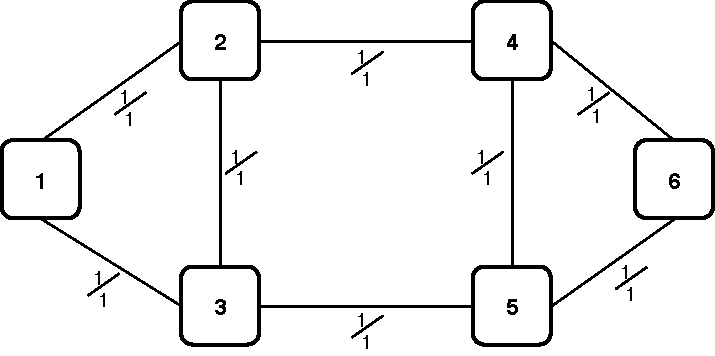
\includegraphics[width=13cm]{sdf/ilp/transparent_protection/figures/physical_topology}
\caption{Transparent with 1+1 protection in medium scenario: Physical topology after dimensioning.}
\label{physical2_protectionmedium}
\end{figure}

\newpage
\begin{figure}[h!]
\centering
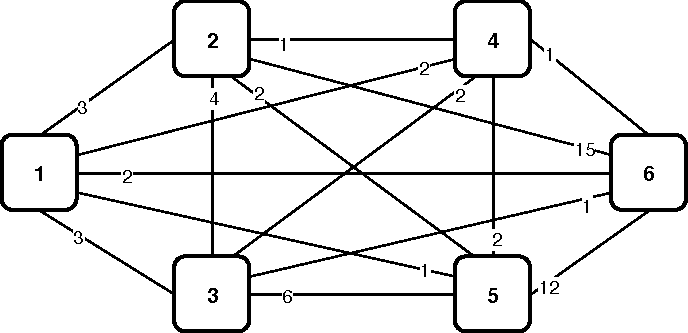
\includegraphics[width=13cm]{sdf/ilp/transparent_protection/figures/optical_topology_medium}
\caption{Transparent with 1+1 protection in medium scenario: Optical topology after dimensioning.}
\label{optical2_protectionmedium}
\end{figure}

\vspace{15pt}
In table \ref{link_transp_protec_ref_medium} we can see the number of optical channels calculated using \ref{Capex_Link} and \ref{ILPOpaque_CAPEX} and the number of amplifiers for each link calculated using \ref{Capex_amplifiers}.\\

\begin{table}[h!]
\centering
\begin{tabular}{|| c | c | c ||}
 \hline
 \multicolumn{3}{|| c ||}{Information regarding links} \\
 \hline
 \hline
 Bidirectional Link & Optical Channels & Amplifiers\\
 \hline
 Node 1 <-> Node 2 & 15 & 4 \\
 Node 1 <-> Node 3 & 15 & 6 \\
 Node 2 <-> Node 3 & 37 & 0 \\
 Node 2 <-> Node 4 & 32 & 6 \\
 Node 3 <-> Node 5 & 32 & 8 \\
 Node 4 <-> Node 5 & 29 & 1 \\
 Node 4 <-> Node 6 & 33 & 7 \\
 Node 5 <-> Node 6 & 33 & 3 \\
 \hline
\end{tabular}
\caption{Table with information regarding links for transparent mode with 1+1 protection.}
\label{link_transp_protec_ref_medium}
\end{table}

\vspace{15pt}
In table \ref{node_transp_protec_ref_medium} we can see the resulting nodal degree at the physical layer, the number of line ports and the number of add ports for the optical part calculated using \ref{OXC_poxc_transparent} the number of LR transponders calculated using \ref{EXC_pexc2_transparent} and the number of tributary ports calculated using \ref{EXC_pexc1_transparent} for each node.\\
\newpage
\begin{table}[h!]
\centering
\begin{tabular}{|| c | c | c | c | c | c ||}
 \hline
 \multicolumn{6}{|| c ||}{Information regarding nodes} \\
 \hline
 \hline
 \multicolumn{2}{|| c |}{ } & \multicolumn{2}{ c |}{Electrical part} & \multicolumn{2}{ c ||}{Optical part} \\
 \hline
 Node & Resulting Nodal Degree & Tributary Ports & LR Transponders & Add Ports & Line Ports\\
 \hline
 1 & 2 & 290 & 11 & 11 & 30 \\
 2 & 3 & 230 & 25 & 25 & 84 \\
 3 & 3 & 180 & 16 & 16 & 84 \\
 4 & 3 & 200 & 8 & 8 & 94 \\
 5 & 3 & 240 & 23 & 23 & 94 \\
 6 & 2 & 220 & 31 & 31 & 66 \\
\hline
\end{tabular}
\caption{Table with information regarding nodes for transparent mode with 1+1 protection.}
\label{node_transp_protec_ref_medium}
\end{table}

Through the information obtained previously on the nodes we can now create tables with detailed information about each node.\\

\begin{table}[h!]
\centering
\begin{tabular}{|| c | c | c ||}
 \hline
 \multicolumn{3}{|| c ||}{Detailed description of Node 1} \\
 \hline
 \hline
 Electrical part & Number of tributary ports & Bit rate \\ \hline
\multirow{3}{*}{290 tributary ports} & 130 & ODU0 \\
 & 130 & ODU1 \\
 & 30 & ODU2 \\
 \hline
  & Node<--Optical Channels-->Node & Bit rate \\
 \hline
 \multirow{5}{*}{11 LR Transponders} & 1  <---- 3 ---->  2 & \multirow{5}{*}{100 Gbits/s} \\
  & 1  <---- 3 ---->  3 & \\
  & 1  <---- 2 ---->  4 & \\
  & 1  <---- 1 ---->  5 & \\
  & 1  <---- 2 ---->  6 & \\
 \hline
 \hline
 Optical part & Node<--Optical Channels-->Node & Bit rate \\
 \hline
 \multirow{5}{*}{11 add ports} & 1  <---- 3 ---->  2 & \multirow{11}{*}{100 Gbits/s} \\
  & 1  <---- 3 ---->  3 & \\
  & 1  <---- 2 ---->  4 & \\
  & 1  <---- 1 ---->  5 & \\
  & 1  <---- 2 ---->  6 & \\ \cline{1-2}
 \multirow{6}{*}{30 line ports} & 1  <---- 3 ---->  2 & \\
  & 1  <---- 3 ---->  3 & \\
  & 1  <---- 2 ---->  4 & \\
  & 1  <---- 1 ---->  5 & \\
  & 1  <---- 2 ---->  6 & \\
  & 2  <---- 4 ---->  3 & \\
\hline
\end{tabular}
\caption{Transparent with 1+1 protection in medium scenario: Detailed description of node 1. The number of demands is distributed to the various destination nodes, this distribution can be observed in section \ref{medium_traffic_scenario}. Regarding the number of line ports when this node is equal to the source, it means that add ports are used, otherwise it means that through ports are used.}
\end{table}

\newpage
\begin{table}[h!]
\centering
\begin{tabular}{|| c | c | c ||}
 \hline
 \multicolumn{3}{|| c ||}{Detailed description of Node 2} \\
 \hline
 \hline
 Electrical part & Number of tributary ports & Bit rate \\ \hline
\multirow{5}{*}{230 tributary ports} & 110 & ODU0 \\
 & 70 & ODU1 \\
 & 20 & ODU2 \\
 & 20 & ODU3 \\
 & 10 & ODU4 \\
 \hline
  & Node<--Optical Channels-->Node & Bit rate \\
 \hline
 \multirow{5}{*}{25 LR Transponders} & 2  <---- 3 ---->  1 & \multirow{5}{*}{100 Gbits/s} \\
  & 2  <---- 4 ---->  3 & \\
  & 2  <---- 1 ---->  4 & \\
  & 2  <---- 2 ---->  5 & \\
  & 2  <---- 15 ---->  6 & \\
 \hline
 \hline
 Optical part & Node<--Optical Channels-->Node & Bit rate \\
 \hline
 \multirow{5}{*}{25 add ports} & 2  <---- 3 ---->  1 & \multirow{17}{*}{100 Gbits/s} \\
  & 2  <---- 4 ---->  3 & \\
  & 2  <---- 1 ---->  4 & \\
  & 2  <---- 2 ---->  5 & \\
  & 2  <---- 15 ---->  6 & \\ \cline{1-2}
 \multirow{12}{*}{84 line ports} & 2  <---- 3 ---->  1 & \\
  & 2  <---- 4 ---->  3 & \\
  & 2  <---- 1 ---->  4 & \\
  & 2  <---- 2 ---->  5 & \\
  & 2  <---- 15 ---->  6 & \\
  & 1  <---- 3 ---->  3 & \\
  & 1  <---- 2 ---->  4 & \\
  & 1  <---- 1 ---->  5 & \\
  & 1  <---- 2 ---->  6 & \\
  & 3  <---- 2 ---->  4 & \\
  & 3  <---- 6 ---->  5 & \\
  & 3  <---- 1 ---->  6 & \\
\hline
\end{tabular}
\caption{Transparent with 1+1 protection in medium scenario: Detailed description of node 2. The number of demands is distributed to the various destination nodes, this distribution can be observed in section \ref{medium_traffic_scenario}. Regarding the number of line ports when this node is equal to the source, it means that add ports are used, otherwise it means that through ports are used. In both cases the number of ports is double the number of optical channels.}
\end{table}

\newpage
\begin{table}[h!]
\centering
\begin{tabular}{|| c | c | c ||}
 \hline
 \multicolumn{3}{|| c ||}{Detailed description of Node 3} \\
 \hline
 \hline
 Electrical part & Number of tributary ports & Bit rate \\ \hline
\multirow{4}{*}{180 tributary ports} & 70 & ODU0 \\
 & 60 & ODU1\\
 & 30 & ODU2\\
 & 20 & ODU3\\
 \hline
  & Node<--Optical Channels-->Node & Bit rate \\
 \hline
 \multirow{5}{*}{16 LR Transponders} & 3  <---- 3 ---->  1 & \multirow{5}{*}{100 Gbits/s} \\
  & 3  <---- 4 ---->  2 & \\
  & 3  <---- 2 ---->  4 & \\
  & 3  <---- 6 ---->  5 & \\
  & 3  <---- 1 ---->  6 & \\
 \hline
 \hline
 Optical part & Node<--Optical Channels-->Node & Bit rate \\
 \hline
 \multirow{5}{*}{16 add ports} & 3  <---- 3 ---->  1 & \multirow{17}{*}{100 Gbits/s} \\
  & 3  <---- 4 ---->  2 & \\
  & 3  <---- 2 ---->  4 & \\
  & 3  <---- 6 ---->  5 & \\
  & 3  <---- 1 ---->  6 & \\ \cline{1-2}
 \multirow{12}{*}{84 line ports} & 3  <---- 3 ---->  1 & \\
  & 3  <---- 4 ---->  2 & \\
  & 3  <---- 2 ---->  4 & \\
  & 3  <---- 6 ---->  5 & \\
  & 3  <---- 1 ---->  6 & \\
  & 1  <---- 3 ---->  2 & \\
  & 1  <---- 2 ---->  4 & \\
  & 1  <---- 1 ---->  5 & \\
  & 1  <---- 2 ---->  6 & \\
  & 2  <---- 1 ---->  4 & \\
  & 2  <---- 2 ---->  5 & \\
  & 2  <---- 15 ---->  6 & \\
\hline
\end{tabular}
\caption{Transparent with 1+1 protection in medium scenario: Detailed description of node 3. The number of demands is distributed to the various destination nodes, this distribution can be observed in section \ref{medium_traffic_scenario}. Regarding the number of line ports when this node is equal to the source, it means that add ports are used, otherwise it means that through ports are used. In both cases the number of ports is double the number of optical channels.}
\end{table}

\newpage
\begin{table}[h!]
\centering
\begin{tabular}{|| c | c | c ||}
 \hline
 \multicolumn{3}{|| c ||}{Detailed description of Node 4} \\
 \hline
 \hline
 Electrical part & Number of tributary ports & Bit rate \\ \hline
\multirow{3}{*}{200 tributary ports} & 70 & ODU0 \\
 & 100 & ODU1 \\
 & 30 & ODU2 \\
 \hline
  & Node<--Optical Channels-->Node & Bit rate \\
 \hline
 \multirow{5}{*}{8 LR Transponders} & 4  <---- 2 ---->  1 & \multirow{5}{*}{100 Gbits/s} \\
  & 4  <---- 1 ---->  2 & \\
  & 4  <---- 2 ---->  3 & \\
  & 4  <---- 2 ---->  5 & \\
  & 4  <---- 1 ---->  6 & \\
 \hline
 \hline
 Optical part & Node<--Optical Channels-->Node & Bit rate \\
 \hline
 \multirow{5}{*}{8 add ports} & 4  <---- 2 ---->  1 & \multirow{17}{*}{100 Gbits/s} \\
  & 4  <---- 1 ---->  2 & \\
  & 4  <---- 2 ---->  3 & \\
  & 4  <---- 2 ---->  5 & \\
  & 4  <---- 1 ---->  6 & \\ \cline{1-2}
 \multirow{12}{*}{94 line ports} & 4  <---- 2 ---->  1 & \\
  & 4  <---- 1 ---->  2 & \\
  & 4  <---- 2 ---->  3 & \\
  & 4  <---- 2 ---->  5 & \\
  & 4  <---- 1 ---->  6 & \\
  & 1  <---- 1 ---->  5 & \\
  & 1  <---- 2 ---->  6 & \\
  & 2  <---- 2 ---->  5 & \\
  & 2  <---- 15 ---->  6 & \\
  & 3  <---- 6 ---->  5 & \\
  & 3  <---- 1 ---->  6 & \\
  & 5  <---- 12 ---->  6 & \\
\hline
\end{tabular}
\caption{Transparent with 1+1 protection in medium scenario: Detailed description of node 4. The number of demands is distributed to the various destination nodes, this distribution can be observed in section \ref{medium_traffic_scenario}. Regarding the number of line ports when this node is equal to the source, it means that add ports are used, otherwise it means that through ports are used. In both cases the number of ports is double the number of optical channels.}
\end{table}

\newpage
\begin{table}[h!]
\centering
\begin{tabular}{|| c | c | c ||}
 \hline
 \multicolumn{3}{|| c ||}{Detailed description of Node 5} \\
 \hline
 \hline
 Electrical part & Number of tributary ports & Bit rate \\ \hline
\multirow{5}{*}{240 tributary ports} & 140 & ODU0 \\
 & 40 & ODU1 \\
 & 40 & ODU2 \\
 & 10 & ODU3 \\
 & 10 & ODU4 \\
 \hline
  & Node<--Optical Channels-->Node & Bit rate \\
 \hline
 \multirow{5}{*}{23 LR Transponders} & 5  <---- 1 ---->  1 & \multirow{5}{*}{100 Gbits/s} \\
  & 5  <---- 2 ---->  2 & \\
  & 5  <---- 6 ---->  3 & \\
  & 5  <---- 2 ---->  4 & \\
  & 5  <---- 12 ---->  6 & \\
 \hline
 \hline
 Optical part & Node<--Optical Channels-->Node & Bit rate \\
 \hline
 \multirow{5}{*}{23 add ports} & 5  <---- 1 ---->  1 & \multirow{17}{*}{100 Gbits/s} \\
  & 5  <---- 2 ---->  2 & \\
  & 5  <---- 6 ---->  3 & \\
  & 5  <---- 2 ---->  4 & \\
  & 5  <---- 12 ---->  6 & \\ \cline{1-2}
 \multirow{12}{*}{94 line ports} & 5  <---- 1 ---->  1 & \\
  & 5  <---- 2 ---->  2 & \\
  & 5  <---- 6 ---->  3 & \\
  & 5  <---- 2 ---->  4 & \\
  & 5  <---- 12 ---->  6 & \\
  & 1  <---- 2 ---->  4 & \\
  & 1  <---- 2 ---->  6 & \\
  & 2  <---- 1 ---->  4 & \\
  & 2  <---- 15 ---->  6 & \\
  & 3  <---- 2 ---->  4 & \\
  & 3  <---- 1 ---->  6 & \\
  & 4  <---- 1 ---->  6 & \\
\hline
\end{tabular}
\caption{Transparent with 1+1 protection in medium scenario: Detailed description of node 5. The number of demands is distributed to the various destination nodes, this distribution can be observed in section \ref{medium_traffic_scenario}. Regarding the number of line ports when this node is equal to the source, it means that add ports are used, otherwise it means that through ports are used. In both cases the number of ports is double the number of optical channels.}
\end{table}

\newpage
\begin{table}[h!]
\centering
\begin{tabular}{|| c | c | c ||}
 \hline
 \multicolumn{3}{|| c ||}{Detailed description of Node 6} \\
 \hline
 \hline
 Electrical part & Number of tributary ports & Bit rate \\ \hline
\multirow{5}{*}{220 tributary ports} & 80 & ODU0 \\
 & 100 & ODU1 \\
 & 10 & ODU2 \\
 & 10 & ODU3 \\
 & 20 & ODU4 \\
 \hline
  & Node<--Optical Channels-->Node & Bit rate \\
 \hline
 \multirow{5}{*}{31 LR Transponders} & 6  <---- 2 ---->  1 & \multirow{5}{*}{100 Gbits/s} \\
  & 6  <---- 15 ---->  2 & \\
  & 6  <---- 1 ---->  3 & \\
  & 6  <---- 1 ---->  4 & \\
  & 6  <---- 12 ---->  5 & \\
 \hline
 \hline
 Optical part & Node<--Optical Channels-->Node & Bit rate \\
 \hline
 \multirow{5}{*}{31 add ports} & 6  <---- 2 ---->  1 & \multirow{11}{*}{100 Gbits/s} \\
  & 6  <---- 15 ---->  2 & \\
  & 6  <---- 1 ---->  3 & \\
  & 6  <---- 1 ---->  4 & \\
  & 6  <---- 12 ---->  5 & \\ \cline{1-2}
 \multirow{6}{*}{66 line ports} & 6  <---- 2 ---->  1 & \\
  & 6  <---- 15 ---->  2 & \\
  & 6  <---- 1 ---->  3 & \\
  & 6  <---- 1 ---->  4 & \\
  & 6  <---- 12 ---->  5 & \\
  & 4  <---- 2 ---->  5 & \\
\hline
\end{tabular}
\caption{Transparent with 1+1 protection in medium scenario: Detailed description of node 6. The number of demands is distributed to the various destination nodes, this distribution can be observed in section \ref{medium_traffic_scenario}. Regarding the number of line ports when this node is equal to the source, it means that add ports are used, otherwise it means that through ports are used. In both cases the number of ports is double the number of optical channels.}
\end{table}

In next step let's focus on the routing information. These paths are bidirectional so the path from one node to another is the same path in the opposite direction. In table \ref{path_transp_protec_ref_medium} we can see all the routing obtained for all nodes.\\
\newpage
\begin{table}[h!]
\centering
\begin{tabular}{|| c | c | c ||}
 \hline
 \multicolumn{3}{|| c ||}{Routing} \\
 \hline
 \hline
 o & d & Links \\
 \hline
 \multirow{2}{*}{1} & \multirow{2}{*}{2} & \{(1,3),(3,2)\} \\
 & & \{(1,2)\} \\ \hline
 \multirow{2}{*}{1} & \multirow{2}{*}{3} & \{(1,2),(2,3)\} \\
 & & \{(1,3)\} \\ \hline
 \multirow{2}{*}{1} & \multirow{2}{*}{4} & \{(1,3),(3,5),(5,4)\} \\
 & & \{(1,2),(2,4)\} \\ \hline
 \multirow{2}{*}{1} & \multirow{2}{*}{5} & \{(1,2),(2,4),(4,5)\} \\
 & & \{(1,3),(3,5)\} \\ \hline
 \multirow{2}{*}{1} & \multirow{2}{*}{6} & \{(1,3),(3,5),(5,6)\} \\
 & & \{(1,2),(2,4),(4,6)\} \\ \hline
 \multirow{2}{*}{2} & \multirow{2}{*}{3} & \{(2,1),(1,3)\} \\
 & & \{(2,3)\} \\ \hline
 \multirow{2}{*}{2} & \multirow{2}{*}{4} & \{(2,3),(3,5),(5,4)\} \\
 & & \{(2,4)\} \\ \hline
 \multirow{2}{*}{2} & \multirow{2}{*}{5} & \{(2,4),(4,5)\} \\
 & & \{(2,3),(3,5)\} \\ \hline
 \multirow{2}{*}{2} & \multirow{2}{*}{6} & \{(2,3),(3,5),(5,6)\} \\
 & & \{(2,4),(4,6)\} \\ \hline
 \multirow{2}{*}{3} & \multirow{2}{*}{4} & \{(3,5),(5,4)\} \\
 & & \{(3,2),(2,4)\} \\ \hline
 \multirow{2}{*}{3} & \multirow{2}{*}{5} & \{(3,2),(2,4),(4,5)\} \\
 & & \{(3,5)\} \\ \hline
 \multirow{2}{*}{3} & \multirow{2}{*}{6} & \{(3,2),(2,4),(4,6)\} \\
 & & \{(3,5),(5,6)\} \\ \hline
 \multirow{2}{*}{4} & \multirow{2}{*}{5} & \{(4,6),(6,5)\} \\
 & & \{(4,5)\} \\ \hline
 \multirow{2}{*}{4} & \multirow{2}{*}{6} & \{(4,5),(5,6)\} \\
 & & \{(4,6)\} \\ \hline
 \multirow{2}{*}{5} & \multirow{2}{*}{6} & \{(5,4),(4,6)\} \\
 & & \{(5,6)\} \\
 \hline
\end{tabular}
\caption{Transparent with 1+1 protection in medium scenario: Description of routing.}
\label{path_transp_protec_ref_medium}
\end{table}

Finally and most importantly through table \ref{scripttransp_protec_ref_medium} we can see the CAPEX result for this model. This value is obtained using equation \ref{ILPOpaque_CAPEX} and all of the constraints mentioned above.\\
\newpage
\begin{table}[h!]
\centering
\begin{tabular}{|| c | c | c | c | c | c | c ||}
 \hline
 \multicolumn{7}{|| c ||}{CAPEX of the Network} \\
 \hline
 \hline
 \multicolumn{3}{|| c |}{ } & Quantity & Unit Price & Cost & Total \\
 \hline
 \multirow{3}{*}{Link Cost} & \multicolumn{2}{ c |}{OLTs} & 16 & 15 000 \euro & 240 000 \euro & \multirow{3}{*}{226 520 000 \euro} \\ \cline{2-6}
 &\multicolumn{2}{ c |}{100 Gbits/s Transceivers}& 452 & 5 000 \euro/Gbit/s &226 000 000 \euro& \\ \cline{2-6}
 & \multicolumn{2}{ c |}{Amplifiers} & 70 & 4 000 \euro & 280 000 \euro & \\
 \hline
 \multirow{10}{*}{Node Cost} & \multirow{7}{*}{Electrical} & EXCs & 6 & 10 000 \euro & 60 000 \euro & \multirow{10}{*}{13 020 900 \euro} \\ \cline{3-6}
 & & ODU0 Ports & 600 & 10 \euro/port & 6 000 \euro & \\ \cline{3-6}
 & & ODU1 Ports & 500 & 15 \euro/port & 7 500 \euro & \\ \cline{3-6}
 & & ODU2 Ports & 160 & 30 \euro/port & 4 800 \euro & \\ \cline{3-6}
 & & ODU3 Ports & 60 & 60 \euro/port & 3 600 \euro & \\ \cline{3-6}
 & & ODU4 Ports & 40 & 100 \euro/port & 4 000 \euro & \\ \cline{3-6}
 & &Transponders& 114 &100 000 \euro/port& 11 400 000 \euro & \\ \cline{2-6}
 & \multirow{3}{*}{Optical} & OXCs & 6 & 20 000 \euro & 120 000 \euro & \\ \cline{3-6}
 & & Line Ports & 452 & 2 500 \euro/port & 1 130 000 \euro & \\ \cline{3-6}
 & & Add Ports & 114 & 2 500 \euro/port & 285 000 \euro & \\
 \hline
 \multicolumn{6}{|| c |}{Total Network Cost} &239 540 900 \euro\\
\hline
\end{tabular}
\caption{Transparent with 1+1 protection in medium scenario: Detailed description of CAPEX for this scenario.}
\label{scripttransp_protec_ref_medium}
\end{table}


\textbf{High Traffic Scenario:}\\

In this scenario we have to take into account the traffic calculated in \ref{high_traffic_scenario}. In a first phase, we will show the resulting physical and optical topology. These topologies are based on the allowed topologies referred to in the model description and also taking into account the logical topology for all ODU's mentioned in the section \ref{high_traffic_scenario}.\\

\begin{figure}[h!]
\centering
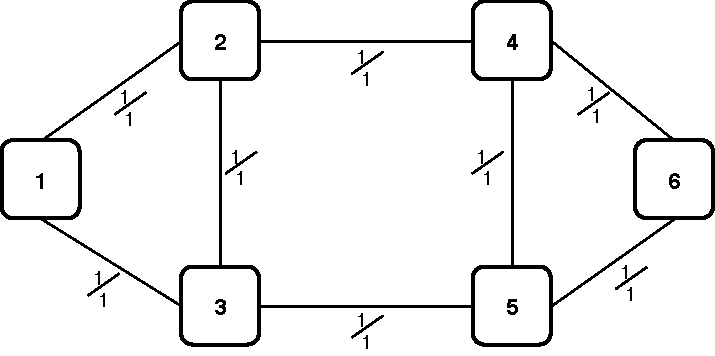
\includegraphics[width=13cm]{sdf/ilp/transparent_protection/figures/physical_topology}
\caption{Transparent with 1+1 protection in high scenario: Physical topology after dimensioning.}
\label{physical2_protectionhigh}
\end{figure}

\newpage
\begin{figure}[h!]
\centering
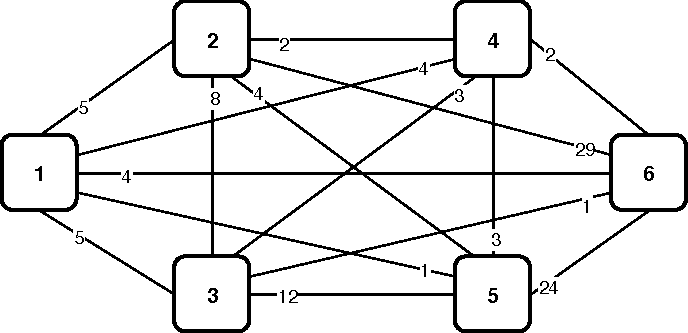
\includegraphics[width=13cm]{sdf/ilp/transparent_protection/figures/optical_topology_high}
\caption{Transparent with 1+1 protection in high scenario: Optical topology after dimensioning.}
\label{optical2_protectionhigh}
\end{figure}

\vspace{15pt}
In table \ref{link_transp_protec_ref_high} we can see the number of optical channels calculated using \ref{Capex_Link} and \ref{ILPOpaque_CAPEX} and the number of amplifiers for each link calculated using \ref{Capex_amplifiers}.\\

\begin{table}[h!]
\centering
\begin{tabular}{|| c | c | c ||}
 \hline
 \multicolumn{3}{|| c ||}{Information regarding links} \\
 \hline
 \hline
 Bidirectional Link & Optical Channels & Amplifiers\\
 \hline
 Node 1 <-> Node 2 & 27 & 4 \\
 Node 1 <-> Node 3 & 27 & 6 \\
 Node 2 <-> Node 3 & 69 & 0 \\
 Node 2 <-> Node 4 & 60 & 6 \\
 Node 3 <-> Node 5 & 60 & 8 \\
 Node 4 <-> Node 5 & 55 & 1 \\
 Node 4 <-> Node 6 & 63 & 7 \\
 Node 5 <-> Node 6 & 63 & 3 \\
 \hline
\end{tabular}
\caption{Table with information regarding links for transparent mode with 1+1 protection in high scenario.}
\label{link_transp_protec_ref_high}
\end{table}

\vspace{15pt}
In table \ref{node_transp_protec_ref_high} we can see the resulting nodal degree at the physical layer, the number of line ports and the number of add ports for the optical part calculated using \ref{OXC_poxc_transparent} the number of LR transponders calculated using \ref{EXC_pexc2_transparent} and the number of tributary ports calculated using \ref{EXC_pexc1_transparent} for each node.\\

\newpage
\begin{table}[h!]
\centering
\begin{tabular}{|| c | c | c | c | c | c ||}
 \hline
 \multicolumn{6}{|| c ||}{Information regarding nodes} \\
 \hline
 \hline
 \multicolumn{2}{|| c |}{ } & \multicolumn{2}{ c |}{Electrical part} & \multicolumn{2}{ c ||}{Optical part} \\
 \hline
 Node & Resulting Nodal Degree & Tributary Ports & LR Transponders & Add Ports & Line Ports\\
 \hline
 1 & 2 & 580 & 19 & 19 & 54 \\
 2 & 3 & 460 & 48 & 48 & 156 \\
 3 & 3 & 360 & 29 & 29 & 156 \\
 4 & 3 & 400 & 14 & 14 & 178 \\
 5 & 3 & 480 & 44 & 44 & 178 \\
 6 & 2 & 440 & 60 & 60 & 126 \\
\hline
\end{tabular}
\caption{Table with information regarding nodes for transparent mode with 1+1 protection in high scenario.}
\label{node_transp_protec_ref_high}
\end{table}

Through the information obtained previously on the nodes we can now create tables with detailed information about each node.\\

\begin{table}[h!]
\centering
\begin{tabular}{|| c | c | c ||}
 \hline
 \multicolumn{3}{|| c ||}{Detailed description of Node 1} \\
 \hline
 \hline
 Electrical part & Number of tributary ports & Bit rate \\ \hline
\multirow{3}{*}{580 tributary ports} & 260 & ODU0 \\
 & 260 & ODU1 \\
 & 60 & ODU2 \\
 \hline
  & Node<--Optical Channels-->Node & Bit rate \\
 \hline
 \multirow{5}{*}{19 LR Transponders} & 1  <---- 5 ---->  2 & \multirow{5}{*}{100 Gbits/s} \\
  & 1  <---- 5 ---->  3 & \\
  & 1  <---- 4 ---->  4 & \\
  & 1  <---- 1 ---->  5 & \\
  & 1  <---- 4 ---->  6 & \\
 \hline
 \hline
 Optical part & Node<--Optical Channels-->Node & Bit rate \\
 \hline
 \multirow{5}{*}{19 add ports} & 1  <---- 5 ---->  2 & \multirow{11}{*}{100 Gbits/s} \\
  & 1  <---- 5 ---->  3 & \\
  & 1  <---- 4 ---->  4 & \\
  & 1  <---- 1 ---->  5 & \\
  & 1  <---- 4 ---->  6 & \\ \cline{1-2}
 \multirow{6}{*}{54 line ports} & 1  <---- 5 ---->  2 & \\
  & 1  <---- 5 ---->  3 & \\
  & 1  <---- 4 ---->  4 & \\
  & 1  <---- 1 ---->  5 & \\
  & 1  <---- 4 ---->  6 & \\
  & 2  <---- 8 ---->  3 & \\
\hline
\end{tabular}
\caption{Transparent with 1+1 protection in high scenario: Detailed description of node 1. The number of demands is distributed to the various destination nodes, this distribution can be observed in section \ref{high_traffic_scenario} . Regarding the number of line ports when this node is equal to the source, it means that add ports are used, otherwise it means that through ports are used.}
\end{table}

\newpage
\begin{table}[h!]
\centering
\begin{tabular}{|| c | c | c ||}
 \hline
 \multicolumn{3}{|| c ||}{Detailed description of Node 2} \\
 \hline
 \hline
 Electrical part & Number of tributary ports & Bit rate \\ \hline
\multirow{5}{*}{460 tributary ports} & 220 & ODU0 \\
 & 140 & ODU1 \\
 & 40 & ODU2 \\
 & 40 & ODU3 \\
 & 20 & ODU4 \\
 \hline
  Node<--Optical Channels-->Node & Bit rate \\
 \hline
 \multirow{5}{*}{48 LR Transponders} & 2  <---- 5 ---->  1 & \multirow{5}{*}{100 Gbits/s} \\
  & 2  <---- 8 ---->  3 & \\
  & 2  <---- 2 ---->  4 & \\
  & 2  <---- 4 ---->  5 & \\
  & 2  <---- 29 ---->  6 & \\
 \hline
 \hline
 Optical part & Node<--Optical Channels-->Node & Bit rate \\
 \hline
 \multirow{5}{*}{48 add ports} & 2  <---- 5 ---->  1 & \multirow{17}{*}{100 Gbits/s} \\
  & 2  <---- 8 ---->  3 & \\
  & 2  <---- 2 ---->  4 & \\
  & 2  <---- 4 ---->  5 & \\
  & 2  <---- 29 ---->  6 & \\ \cline{1-2}
 \multirow{12}{*}{156 line ports} & 2  <---- 5 ---->  1 & \\
  & 2  <---- 8 ---->  3 & \\
  & 2  <---- 2 ---->  4 & \\
  & 2  <---- 4 ---->  5 & \\
  & 2  <---- 29 ---->  6 & \\
  & 1  <---- 5 ---->  3 & \\
  & 1  <---- 4 ---->  4 & \\
  & 1  <---- 1 ---->  5 & \\
  & 1  <---- 4 ---->  6 & \\
  & 3  <---- 3 ---->  4 & \\
  & 3  <---- 12 ---->  5 & \\
  & 3  <---- 1 ---->  6  & \\
\hline
\end{tabular}
\caption{Transparent with 1+1 protection in high scenario: Detailed description of node 2. The number of demands is distributed to the various destination nodes, this distribution can be observed in section \ref{high_traffic_scenario} . Regarding the number of line ports when this node is equal to the source, it means that add ports are used, otherwise it means that through ports are used. In both cases the number of ports is double the number of optical channels.}
\end{table}

\newpage
\begin{table}[h!]
\centering
\begin{tabular}{|| c | c | c ||}
 \hline
 \multicolumn{3}{|| c ||}{Detailed description of Node 3} \\
 \hline
 \hline
 Electrical part & Number of tributary ports & Bit rate \\ \hline
\multirow{4}{*}{360 tributary ports} & 140 & ODU0 \\
 & 120 & ODU1\\
 & 60 & ODU2\\
 & 40 & ODU3\\
 \hline
  & Node<--Optical Channels-->Node & Bit rate \\
 \hline
 \multirow{5}{*}{29 LR Transponders} & 3  <---- 5 ---->  1 & \multirow{5}{*}{100 Gbits/s} \\
  & 3  <---- 8 ---->  2 & \\
  & 3  <---- 3 ---->  4 & \\
  & 3  <---- 12 ---->  5 & \\
  & 3  <---- 1 ---->  6 & \\
 \hline
 \hline
 Optical part & Node<--Optical Channels-->Node & Bit rate \\
 \hline
 \multirow{5}{*}{29 add ports} & 3  <---- 5 ---->  1 & \multirow{17}{*}{100 Gbits/s} \\
  & 3  <---- 8 ---->  2 & \\
  & 3  <---- 3 ---->  4 & \\
  & 3  <---- 12 ---->  5 & \\
  & 3  <---- 1 ---->  6 & \\ \cline{1-2}
 \multirow{12}{*}{156 line ports} & 3  <---- 5 ---->  1 & \\
  & 3  <---- 8 ---->  2 & \\
  & 3  <---- 3 ---->  4 & \\
  & 3  <---- 12 ---->  5 & \\
  & 3  <---- 1 ---->  6 & \\
  & 1  <---- 5 ---->  2 & \\
  & 1  <---- 4 ---->  4 & \\
  & 1  <---- 1 ---->  5 & \\
  & 1  <---- 4 ---->  6 & \\
  & 2  <---- 2 ---->  4 & \\
  & 2  <---- 4 ---->  5 & \\
  & 2  <---- 29 ---->  6 & \\
\hline
\end{tabular}
\caption{Transparent with 1+1 protection in high scenario: Detailed description of node 3. The number of demands is distributed to the various destination nodes, this distribution can be observed in section \ref{high_traffic_scenario} . Regarding the number of line ports when this node is equal to the source, it means that add ports are used, otherwise it means that through ports are used. In both cases the number of ports is double the number of optical channels.}
\end{table}

\newpage
\begin{table}[h!]
\centering
\begin{tabular}{|| c | c | c ||}
 \hline
 \multicolumn{3}{|| c ||}{Detailed description of Node 4} \\
 \hline
 \hline
 Electrical part & Number of tributary ports & Bit rate \\ \hline
\multirow{3}{*}{400 tributary ports} & 140 & ODU0 \\
 & 200 & ODU1 \\
 & 60 & ODU2 \\
 \hline
  & Node<--Optical Channels-->Node & Bit rate \\
 \hline
 \multirow{5}{*}{14 LR Transponders} & 4  <---- 4 ---->  1 & \multirow{5}{*}{100 Gbits/s} \\
  & 4  <---- 2 ---->  2 & \\
  & 4  <---- 3 ---->  3 & \\
  & 4  <---- 3 ---->  5 & \\
  & 4  <---- 2 ---->  6 & \\
 \hline
 \hline
 Optical part & Node<--Optical Channels-->Node & Bit rate \\
 \hline
 \multirow{5}{*}{14 add ports} & 4  <---- 4 ---->  1 & \multirow{17}{*}{100 Gbits/s} \\
  & 4  <---- 2 ---->  2 & \\
  & 4  <---- 3 ---->  3 & \\
  & 4  <---- 3 ---->  5 & \\
  & 4  <---- 2 ---->  6 & \\ \cline{1-2}
  \multirow{12}{*}{178 line ports} & 4  <---- 4 ---->  1 & \\
  & 4  <---- 2 ---->  2 & \\
  & 4  <---- 3 ---->  3 & \\
  & 4  <---- 3 ---->  5 & \\
  & 4  <---- 2 ---->  6 & \\
  & 1  <---- 1 ---->  5 & \\
  & 1  <---- 4 ---->  6 & \\
  & 2  <---- 4 ---->  5 & \\
  & 2  <---- 29 ---->  6 & \\
  & 3  <---- 12 ---->  5 & \\
  & 3  <---- 1 ---->  6 & \\
  & 5  <---- 24 ---->  6 & \\
\hline
\end{tabular}
\caption{Transparent with 1+1 protection in high scenario: Detailed description of node 4. The number of demands is distributed to the various destination nodes, this distribution can be observed in section \ref{high_traffic_scenario} . Regarding the number of line ports when this node is equal to the source, it means that add ports are used, otherwise it means that through ports are used. In both cases the number of ports is double the number of optical channels.}
\end{table}

\newpage
\begin{table}[h!]
\centering
\begin{tabular}{|| c | c | c ||}
 \hline
 \multicolumn{3}{|| c ||}{Detailed description of Node 5} \\
 \hline
 \hline
 Electrical part & Number of tributary ports & Bit rate \\ \hline
\multirow{5}{*}{480 tributary ports} & 280 & ODU0 \\
 & 80 & ODU1 \\
 & 80 & ODU2 \\
 & 20 & ODU3 \\
 & 20 & ODU4 \\
 \hline
  Node<--Optical Channels-->Node & Bit rate \\
 \hline
 \multirow{5}{*}{44 LR Transponders} & 5  <---- 1 ---->  1 & \multirow{5}{*}{100 Gbits/s} \\
  & 5  <---- 4 ---->  2 & \\
  & 5  <---- 12 ---->  3 & \\
  & 5  <---- 3 ---->  4 & \\
  & 5  <---- 24 ---->  6 & \\
 \hline
 \hline
 Optical part & Node<--Optical Channels-->Node & Bit rate \\
 \hline
 \multirow{5}{*}{44 add ports} & 5  <---- 1 ---->  1 & \multirow{17}{*}{100 Gbits/s} \\
  & 5  <---- 4 ---->  2 & \\
  & 5  <---- 12 ---->  3 & \\
  & 5  <---- 3 ---->  4 & \\
  & 5  <---- 24 ---->  6 & \\ \cline{1-2}
 \multirow{12}{*}{178 line ports} & 5  <---- 1 ---->  1 & \\
  & 5  <---- 4 ---->  2 & \\
  & 5  <---- 12 ---->  3 & \\
  & 5  <---- 3 ---->  4 & \\
  & 5  <---- 24 ---->  6 & \\
  & 1  <---- 4 ---->  4 & \\
  & 1  <---- 4 ---->  6 & \\
  & 2  <---- 2 ---->  4 & \\
  & 2  <---- 29 ---->  6 & \\
  & 3  <---- 3 ---->  4 & \\
  & 3  <---- 1 ---->  6 & \\
  & 4  <---- 2 ---->  6 & \\
\hline
\end{tabular}
\caption{Transparent with 1+1 protection in high scenario: Detailed description of node 5. The number of demands is distributed to the various destination nodes, this distribution can be observed in section \ref{high_traffic_scenario} . Regarding the number of line ports when this node is equal to the source, it means that add ports are used, otherwise it means that through ports are used. In both cases the number of ports is double the number of optical channels.}
\end{table}

\newpage
\begin{table}[h!]
\centering
\begin{tabular}{|| c | c | c ||}
 \hline
 \multicolumn{3}{|| c ||}{Detailed description of Node 6} \\
 \hline
 \hline
 Electrical part & Number of tributary ports & Bit rate \\ \hline
\multirow{5}{*}{440 tributary ports} & 160 & ODU0 \\
 & 200 & ODU1 \\
 & 20 & ODU2 \\
 & 20 & ODU3 \\
 & 40 & ODU4 \\
 \hline
  & Node<--Optical Channels-->Node & Bit rate \\
 \hline
 \multirow{5}{*}{60 LR Transponders} & 6  <---- 4 ---->  1 & \multirow{5}{*}{100 Gbits/s} \\
  & 6  <---- 29 ---->  2 & \\
  & 6  <---- 1 ---->  3 & \\
  & 6  <---- 2 ---->  4 & \\
  & 6  <---- 24 ---->  5 & \\
 \hline
 \hline
 Optical part & Node<--Optical Channels-->Node & Bit rate \\
 \hline
 \multirow{5}{*}{60 add ports} & 6  <---- 4 ---->  1 & \multirow{11}{*}{100 Gbits/s}\\
  & 6  <---- 29 ---->  2 & \\
  & 6  <---- 1 ---->  3 & \\
  & 6  <---- 2 ---->  4 & \\
  & 6  <---- 24 ---->  5 & \\ \cline{1-2}
  \multirow{6}{*}{126 line ports} & 6  <---- 4 ---->  1 & \\
  & 6  <---- 29 ---->  2 & \\
  & 6  <---- 1 ---->  3 & \\
  & 6  <---- 2 ---->  4 & \\
  & 6  <---- 24 ---->  5 & \\
  & 4  <---- 3 ---->  5 & \\
\hline
\end{tabular}
\caption{Transparent with 1+1 protection in high scenario: Detailed description of node 6. The number of demands is distributed to the various destination nodes, this distribution can be observed in section \ref{high_traffic_scenario} . Regarding the number of line ports when this node is equal to the source, it means that add ports are used, otherwise it means that through ports are used. In both cases the number of ports is double the number of optical channels.}
\end{table}

Now let's focus on the routing information in table \ref{path_transp_protec_ref_high}. These paths are bidirectional so the path from one node to another is the same path in the opposite direction.\\
\newpage

\begin{table}[h!]
\centering
\begin{tabular}{|| c | c | c ||}
 \hline
 \multicolumn{3}{|| c ||}{Routing} \\
 \hline
 \hline
 o & d & Links \\
 \hline
 \multirow{2}{*}{1} & \multirow{2}{*}{2} & \{(1,3),(3,2)\} \\
 & & \{(1,2)\} \\ \hline
 \multirow{2}{*}{1} & \multirow{2}{*}{3} & \{(1,2),(2,3)\} \\
 & & \{(1,3)\} \\ \hline
 \multirow{2}{*}{1} & \multirow{2}{*}{4} & \{(1,3),(3,5),(5,4)\} \\
 & & \{(1,2),(2,4)\} \\ \hline
 \multirow{2}{*}{1} & \multirow{2}{*}{5} & \{(1,2),(2,4),(4,5)\} \\
 & & \{(1,3),(3,5)\} \\ \hline
 \multirow{2}{*}{1} & \multirow{2}{*}{6} & \{(1,3),(3,5),(5,6)\} \\
 & & \{(1,2),(2,4),(4,6)\} \\ \hline
 \multirow{2}{*}{2} & \multirow{2}{*}{3} & \{(2,1),(1,3)\} \\
 & & \{(2,3)\} \\ \hline
 \multirow{2}{*}{2} & \multirow{2}{*}{4} & \{(2,3),(3,5),(5,4)\} \\
 & & \{(2,4)\} \\ \hline
 \multirow{2}{*}{2} & \multirow{2}{*}{5} & \{(2,4),(4,5)\} \\
 & & \{(2,3),(3,5)\} \\ \hline
 \multirow{2}{*}{2} & \multirow{2}{*}{6} & \{(2,3),(3,5),(5,6)\} \\
 & & \{(2,4),(4,6)\} \\ \hline
 \multirow{2}{*}{3} & \multirow{2}{*}{4} & \{(3,5),(5,4)\} \\
 & & \{(3,2),(2,4)\} \\ \hline
 \multirow{2}{*}{3} & \multirow{2}{*}{5} & \{(3,2),(2,4),(4,5)\} \\
 & & \{(3,5)\} \\ \hline
 \multirow{2}{*}{3} & \multirow{2}{*}{6} & \{(3,2),(2,4),(4,6)\} \\
 & & \{(3,5),(5,6)\} \\ \hline
 \multirow{2}{*}{4} & \multirow{2}{*}{5} & \{(4,6),(6,5)\} \\
 & & \{(4,5)\} \\ \hline
 \multirow{2}{*}{4} & \multirow{2}{*}{6} & \{(4,5),(5,6)\} \\
 & & \{(4,6)\} \\ \hline
 \multirow{2}{*}{5} & \multirow{2}{*}{6} & \{(5,4),(4,6)\} \\
 & & \{(5,6)\} \\
 \hline
\end{tabular}
\caption{Transparent with 1+1 protection in high scenario: Description of routing.}
\label{path_transp_protec_ref_high}
\end{table}

Finally and most importantly through table \ref{scripttransp_surv_ref_high} we can see the CAPEX result for this model. This value is obtained using equation \ref{ILPOpaque_CAPEX} and all of the constraints mentioned above.\\
\newpage
\begin{table}[h!]
\centering
\begin{tabular}{|| c | c | c | c | c | c | c ||}
 \hline
 \multicolumn{7}{|| c ||}{CAPEX of the Network} \\
 \hline
 \hline
 \multicolumn{3}{|| c |}{ } & Quantity & Unit Price & Cost & Total \\
 \hline
 \multirow{3}{*}{Link Cost} & \multicolumn{2}{ c |}{OLTs} & 16 & 15 000 \euro & 240 000 \euro & \multirow{3}{*}{424 520 000 \euro} \\ \cline{2-6}
 & \multicolumn{2}{ c |}{100 Gbits/s Transceivers}& 848 & 5 000 \euro/Gbit/s & 424 000 000 \euro & \\ \cline{2-6}
 & \multicolumn{2}{ c |}{Amplifiers} & 70 & 4 000 \euro & 280 000 \euro & \\
 \hline
 \multirow{10}{*}{Node Cost} & \multirow{7}{*}{Electrical} & EXCs & 6 & 10 000 \euro & 60 000 \euro & \multirow{10}{*}{24 286 800 \euro} \\ \cline{3-6}
 & & ODU0 Ports & 1 200 & 10 \euro/port & 12 000 \euro & \\ \cline{3-6}
 & & ODU1 Ports & 1 000 & 15 \euro/port & 15 000 \euro & \\ \cline{3-6}
 & & ODU2 Ports & 320 & 30 \euro/port & 9 600 \euro & \\ \cline{3-6}
 & & ODU3 Ports & 120 & 60 \euro/port & 7 200 \euro & \\ \cline{3-6}
 & & ODU4 Ports & 80 & 100 \euro/port & 8 000 \euro & \\ \cline{3-6}
 & &Transponders& 214 & 100 000 \euro/port & 21 400 000 \euro & \\ \cline{2-6}
 & \multirow{3}{*}{Optical} & OXCs & 6 & 20 000 \euro & 120 000 \euro & \\ \cline{3-6}
 & & Line Ports & 848 & 2 500 \euro/port & 2 120 000 \euro & \\ \cline{3-6}
 & & Add Ports & 214 & 2 500 \euro/port & 535 000 \euro & \\
 \hline
 \multicolumn{6}{|| c |}{Total Network Cost} & 448 806 800 \euro \\
\hline
\end{tabular}
\caption{Transparent with 1+1 protection in high scenario: Detailed description of CAPEX for this scenario.}
\label{scripttransp_protec_ref_high}
\end{table}


\subsection{Conclusions}

Once we have obtained the results for all the scenarios we will now draw some conclusions about these results. For a better analysis of the results will be created the table \ref{table_comparative_transp_surv}.\\

\begin{table}[h!]
\centering
\begin{tabular}{| c | c | c | c |}
 \hline
  & Low Traffic & Medium Traffic  & High Traffic \\
 \hline\hline
 CAPEX without survivability&30 317 590 \euro&96 830 900 \euro&180 471 800 \euro\\ \hline
 CAPEX/Gbit/s without survivability&60 630 \euro/Gbit/s& 19 366 \euro/Gbit/s&18 047 \euro/Gbit/s\\ \hline
 Traffic (Gbit/s) & 500 & 5 000 & 10 000 \\ \hline
 Number of Add ports & 34 & 114 & 214 \\ \hline
 Number of Line ports & 136 & 452 & 848 \\ \hline
 Number of Tributary ports & 138 & 1 380 & 2 760 \\ \hline
 Number of Transceivers & 136 & 452 & 848 \\ \hline
 Number of Transponders & 34 & 114 & 214 \\ \hline
 Link Cost & 68 520 000 \euro & 226 520 000 \euro & 424 520 000 \euro \\ \hline
 Node Cost & 3 947 590 \euro & 13 020 900 \euro & 24 286 800 \euro \\ \hline
 CAPEX & \textbf{72 467 590 \euro} & \textbf{239 540 900\euro} & \textbf{448 806 800 \euro} \\ \hline
 CAPEX/Gbit/s & \textbf{144 935 \euro/Gbit/s} & \textbf{47 908 \euro/Gbit/s} & \textbf{44 880 \euro/Gbit/s}\\
 \hline
\end{tabular}
\caption{Transparent with 1+1 protection in high scenario: Table with different value of CAPEX for this case.}
\label{table_comparative_transp_protec}
\end{table}

\newpage
Looking at the previous table we can make some comparisons between the several scenarios:

\begin{itemize}
    \item Comparing the low traffic scenario with the others, we can see that, despite having an increase of factor ten (average scenario) and factor twenty (high scenario), the same increase does not occur in the final cost (it is lower). This happens because the number of transceivers is smaller than expected (an medium scenario of 1360 would be expected and a high scenario would be expected in 2720);
    \item Comparing the medium traffic scenario with the high traffic scenario, we can see that the factor increase is double and in the final cost this factor is very close but still lower. Again, this happens because the number of transceivers is smaller, but very close to what was expected (the high scenario would be expected at 904);
    \item Comparing the cost with the traffic, we see that, for the low traffic scenario, the cost per traffic is very high in relation to the other two. We can conclude that a low traffic scenario becomes more expensive than a high traffic scenario.
    \item Comparing this cost with the without survivability cost we can conclude that protection is significantly more expensive. As can be seen in the table this increase is more than double as with 1+1 protection we have a cost more than twice than the cost without survivability.
\end{itemize}
